%
% chapter.tex -- Kapitel zur Funktionen, die als Lösungen von Differential-
%                gleichungen definiert sind
%
% (c) 2021 Prof Dr Andreas Müller, Hochschule Rapperswil
%
% !TeX spellcheck = de_CH
\chapter{Differentialgleichungen
\label{buch:chapter:differential}}
\lhead{Differentialgleichungen}
\rhead{}
Allgemeine Sätze über die Existenz und Eindeutigkeit der Lösungen
gewöhnlicher Differentialgleichungen garantieren für fast jeder 
einigermassen vernünftige Gleichung mindestens für kurze Zeit
eine eindeutige Lösung für fast jede Anfangsbedingung.
Die Konstruktion solcher Lösungen stellt sich jedoch als deutlich
schwieriger heraus.

Für einzelne Kategorien von Differentialgleichungen sind 
gut funktionierende Lösungsverfahren gefunden worden, zum Beispiel
für lineare Differentialgleichungen mit konstanten Koeffizienten.
Damit konnten auch Gleichungen gelöst werden, die sich zum Beispiel
durch eine Variablentransformation auf eine lineare Differentialgleichung
mit konstanten Koeffizienten reduzieren lassen, wie die Eulersche
Differentialgleichung.

Die Methode der Separation der Variablen liefert führt die Lösung
einer Differentialgleichung erster Ordnung auf die Bestimmung 
zweier Stammfunktionen und deren Invertierung zurück.
Dieses Verfahren ist jedoch nicht auf Vektordifferentialgleichungen
oder auf Differentialgleichungen höherer Ordnung verallgemeinerungsfähig.

Daneben gibt es eine Reihe von ``Spezialfällen'' wie die
Clairaut-Differentialgleichung oder die damit verwandte
Lagrangesche Differentialgleichung, deren Lösung eine sehr
spezielle Form haben.

Sehr viele Differentialgleichungen in den Anwendungen können aber
mit keinem der genannten Verfahren gelöst werden.
Hier bleibt nichts anderes übrig, als neue spezielle Funktionen
zu definieren, die Lösungen dieser Differentialgleichungen sind.
Dabei ist man bestrebt, möglichst universell einsetzbare Funktionen
zu definieren, die ein breites Anwendungsfeld haben.

In den folgenden Abschnitten wird zunächst gezeigt, dass viele
der bereits bekannten speziellen Funktionen ebenfalls als Lösungen
gewöhnlicher Differentialgleichungen erhalten werden können.
Die numerische Lösung gewöhnlicher Differentialgleichungen ist
oft keine effizientes Vorgehen zur Bestimmung von einzelnen Werten,
daher wird in
Abschnitt~\ref{buch:differentialgleichungen:section:potenzreihenmethode}
eine universelle Methode vorgestellt, mit der eine Potenzreihenentwicklung
gefunden werden kann.
Eine Potenzreihendarstellung ermöglicht nicht nur die Berechnung
einzelner Werte, sondern auch beliebiger Ableitungen und die
analytische Untersuchung der Funktion mit den Methoden der
komplexen Analysis.
Als Beispiel für dieses Verfahren werden in
Abschnitt~\ref{buch:differntialgleichungen:section:bessel}
die Bessel-Funktionen erster Art vorgestellt.

%
% teil2.tex -- Beispiel-File für teil2 
%
% (c) 2020 Prof Dr Andreas Müller, Hochschule Rapperswil
%
\section{Beispiele 
\label{sturmliouville:section:teil2}}
\rhead{Beispiele}


%
% potenzreihenmethode.tex
%
% (c) 2021 Prof Dr Andreas Müller, OST Ostschweizer Fachhochschule
%
\section{Potenzreihenmethode
\label{buch:differentialgleichungen:section:potenzreihenmethode}}
\rhead{Potenzreihenmethode}
Die Potenzreihenmethode versucht die Lösung einer gewöhnlichen
Differentialgleichung als Potenzreihe um die Anfangsbedingung zu
entwickeln.
Wir gehen in diesem Abschnitt von einer Differentialgleichung der
Form
\begin{equation}
b_n(x)y^{(n)}(x)
+
b_{n-1}(x)y^{(n-1)}(x)
+
\dots
+
b_1(x)y'(x)
+
b_0(x)y(x)
=
f(x)
\label{buch:differentialgleichungen:eqn:potenzreihendgl}
\end{equation}
mit der Randbedingung $y(0)=y_0$ aus.
Schon im einfachsten Fall einer homogenen Differentialgleichung erster
Ordnung ergibt sich die Beziehung
\[
b_1(x) y'(x) = b_0(x)y(x),
\]
wobei wir uns $y(x)$ und damit auch $y'(x)$ als Potenzreihe vorstellen.
Insbesondere ist 
\[
\frac{b_1(x)}{b_0(x)} = \frac{y(x)}{y'(x)}
\]
ein Quotient von Potenzreihen, den man natürlich wieder als 
Potenzreihe schreiben kann.
Da es nur auf den Quotienten ankommt, kann man sich auf den Fall
beschränken, dass die Koeffizienten Potenzreihen sind.
Tatsächlich gilt der folgende sehr viel allgemeinere Satz von
Cauchy und Kowalevskaja:

\begin{satz}[Cauchy-Kowalevskaja]
\index{Satz!von Cauchy-Kowalevskaja}%
Eine partielle Differentialgleichung der Ordnung $k$ für eine
Funktion $u(x_1,\dots,x_n,t)=u(x,t)$ 
in expliziter Form
\[
\frac{\partial^k}{\partial t^k}
=
G\biggl(x,t,
\frac{\partial^j\partial^\alpha}{\partial t^j\,\partial x^k}
\biggr)
\quad\text{mit $j<k$ und $|\alpha|+j\le k$}
\]
mit einer Funktion $G$, die analytisch ist in allen Variablen
und der Randbedingung
\[
\frac{\partial^j}{\partial t^j}u(x,0)
=
\varphi_j(x)\quad\text{für $k=0,\dots,k-1$}
\]
mit analytischen Funktion $\varphi_j$ hat eine in einer Umgebung von 
$t=0$ eindeutige analytische Lösung.
\end{satz}

Im folgenden werden wir daher weitere einschränkende Annahmen über
die Koeffizienten $b_k(x)$ machen.

%
% Potenzreihenansatz und Koeffizientenvergleich
%
\subsection{Potenzreihenansatz und Koeffizientenvergleich}
In Abschnitt~\ref{buch:differentialgleichungen:section:beispiele}
wurde von einer grossen Zahl interessanter Funktionen gezeigt, dass
sie einerseits eine Lösungen einer Differentialgleichung sind, 
andererseits aber auch eine Potenzreihendarstellung sind.
Der Satz von Cauchy-Kowalevskaja hat gezeigt, dass dies das zu
erwartende Resultat ist.

Da wir bei einer linearen Differentialgleichung mit analytischen
Koeffizienten eine analytische Lösungsfunktion erwarten dürfen,
können wir auch versuchen, die Lösung der Differentialgleichung
von Anfang an als Potenzreihe
\[
y(x)
=
\sum_{k=0}^{\infty} a_kx^k
\]
anzusetzen.
Die Ableitungen von $y(x)$ sind gleichermassen als Potenzreihen
\begin{align*}
y'(x)
&=
\sum_{k=1}^\infty ka_kx^{k-1}
\\
y''(x)
&=
\sum_{k=2}^\infty k(k-1)a_kx^{k-2}
\\
&\vdots\\
y^{(n)}(x)
&=
\sum_{k=n}^\infty
k(k-1)\cdots(k-n+1) a_kx^{k-n}
=
\sum_{k=n}^\infty
(k-n+1)_n a_k x^{k-n}
=
\sum_{l=0}^\infty
(l+1)_na_{l+n}x^l
\end{align*}
darstellbar.

Der Ansatz für $y(x)$ und seine Ableitungen kann jetzt in die
Differentialgleichung eingsetzt werden.
Durch Ausmultiplizieren wird die Differentialgleichung zu
einer Identität von Potenzreihen.
Zwei Potenzreihen können nur dann übereinstimmen, wenn alle
Koeffizienten übereinstimmen.
So entsteht eine Menge von linearen Gleichungen für die
Koeffizienten $a_k$.
Die Koeffizienten $a_0$ bis $a_{n-1}$ werden gegeben durch die
Anfangswerte der Funktion und der ersten $n-1$ Ableitungen, die
ebenfalls nötig sind, um die Lösungsfunktion eindeutig festzulegen.
Durch Lösen des linearen Gleichungssystems können jetzt die Koeffizienten
und damit die Lösung bestimmt werden.

Setzt man zum Beispiel voraus, dass $b_n(0)\ne 0$ ist, dann ist der
konstante Term
\begin{equation}
b_n(0) n! a_n + b_{n-1}(0) (n-1)! a_{n-1}
+ \dots +
b_2(0) 2! a_2 + b_1(0) a_1 + b_0(0) a_0 = 0.
\label{buch:differntialgleichungen:eqn:konstterm}
\end{equation}
Diese Gleichung ermöglicht, nach $a_n$ aufzulösen:
\[
a_n
=
-
\frac{1}{b_n(0)\,n!}\bigl(
b_{n-1}(0)\,(n-1)!\,a_{n-1} + \dots + 
b_2(0)\,2!\,a_2 + b_1(0)\, a_1 + b_0(0)\, a_0
\bigr).
\]
Falls jedoch der Koeffizient $b_n(x)$ eine Nullstelle bei $x=0$
hat, ist es mit Gleichung~\eqref{buch:differntialgleichungen:eqn:konstterm}
allein nicht möglich, $a_n$ zu bestimmen.

Ein besonders einfacher Fall ist jener, in dem alle Koeffizienten der
Differentialgleichung konstant sind. 
In diesem Fall führen die Koeffizienten von $x^k$ auf die Gleichung
\begin{equation}
b_n n! a_{n+k} + b_{n-1} (n-1)! a_{n-1+k}
+ \dots +
b_2 2! a_{2+k} + b_1 a_{1+k} + b_0 a_{k} = 0.
\label{buch:differntialgleichungen:eqn:kterm}
\end{equation}
für alle $k$.
Die Gleichungen sind also immer lösbar und ergeben
\[
a_{n+k}
=
-
\frac{1}{b_n\,n!}\bigl(
b_{n-1}\,(n-1)!\,a_{n-1+k} + \dots + 
b_2\,2!\,a_{2+k} + b_1\, a_{1+k} + b_0\, a_k
\bigr).
\]



%
% Die Newtonsche Reihe
%
\subsection{Die Newtonsche Reihe
\label{buch:differentialgleichungen:subsection:newtonschereihe}}
Wir lösen die
Differentialgleichung~\eqref{buch:differentialgleichungen:eqn:wurzeldgl1}
mit der Anfangsbedingung $y(t)=1$ mit der Potenzreihenmethode.
Wir setzen daher für die Lösung die Potenzreihe an
\[
y(t)
=
a_0 + a_1t + a_2t^2 + a_3t^3 + \dots + a_kt^k + \dots
\]
Die Ableitung ist
\[
\dot{y}(t)
=
a_1 + 2a_2t + 3a_3t^2 + \dots  + ka_kt^{k-1} + \dots
\]
Einsetzen in die 
Differentialgleichung~\eqref{buch:differentialgleichungen:eqn:wurzeldgl1}
liefert
\begin{align*}
(1+t)
(
a_1 + 2a_2t + 3a_3t^2 + \dots  + ka_kt^{k-1} + \dots
)
&=
\alpha
(
a_0 + a_1t + a_2t^2 + a_3t^3 + \dots + a_kt^k + \dots
)
\\
a_1
+(a_1+2a_2)t
+(2a_2+3a_3)t^2
+(3a_3+4a_4)t^3
+\dots
&=
\alpha a_0 + \alpha a_1t + \alpha a_2t^2 + \alpha a_3t^3 + \dots
\end{align*}
Der Koeffizientenvergleich ergbiet die Gleichungen
\begin{align}
a_1&=\alpha a_0
\notag
\\
a_1+2a_2 &= \alpha a_1 &&\Rightarrow& 2a_2 &= (\alpha-1) a_1
\notag
\\
2a_2+3a_3 &= \alpha a_2&&\Rightarrow& 3a_3 &= (\alpha-2) a_2
\notag
\\
3a_3+4a_4 &= \alpha a_3&&\Rightarrow& 4a_4 &= (\alpha-3) a_3
\notag
\\
4a_4+5a_5 &= \alpha a_4&&\Rightarrow& 5a_5 &= (\alpha-4) a_4
\notag
\\
&\vdots
\notag
\\
&&&& \llap{$(k+1)a_{k+1}$} &= (\alpha-k) a_k
&&\Rightarrow&
a_{k+1} = \frac{\alpha-k}{k+1}a_k.
\label{buch:differentialgleichungen:eqn:newtonreiherekursion}
\end{align}
Die
Rekursionsformel~\eqref{buch:differentialgleichungen:eqn:newtonreiherekursion}
gilt auch im Fall $k=0$.
Aus der Anfangsbedingung folgt $a_0=1$.
Durch wiederholte Anwendung der 
Rekursionsformel~\eqref{buch:differentialgleichungen:eqn:newtonreiherekursion}
erhalten wir jetzt die Koeffizienten
\begin{align*}
a_0&=1
\\
a_1&=\alpha
\\
a_2&=\frac{\alpha(\alpha-1)}{1\cdot 2}
\\
a_3&=\frac{\alpha(\alpha-1)(\alpha-2)}{1\cdot 2\cdot 3}
\\
a_4&=\frac{\alpha(\alpha-1)(\alpha-2)(\alpha-3)}{1\cdot 2\cdot 3\cdot 4}
\\
&\;\vdots
\\
a_k&=\frac{\alpha(\alpha-1)(\alpha-2)\dots(\alpha-k+1)}{k!}.
\end{align*}
Für ganzzahliges $\alpha$ ist $a_k$ der Binomialkoeffizient
\[
a_k=\binom{\alpha}{k}
\]
und $a_k=0$ für $k>\alpha$.
Für nicht ganzzahliges $\alpha$ sind alle Koeffizienten $a_k\ne 0$.

Die Lösung der 
Differentialgleichung~\eqref{buch:differentialgleichungen:eqn:wurzeldgl1}
ist daher die Reihe
\begin{equation}
(1+t)^\alpha
=
\sum_{k=0}^\infty
\frac{\alpha(\alpha-1)\dots(\alpha-k+1)}{k!}\, t^k.
\label{buch:differentialgleichungen:eqn:newtonreihe}
\end{equation}
Für ganzzahliges $\alpha$ wird daraus die binomische Formel
\[
(1+t)^\alpha
=
\sum_{k=0}^\infty
\frac{\alpha(\alpha-1)\dots(\alpha-k+1)}{k!}\, t^k
=
\sum_{k=0}^\alpha \binom{\alpha}{k} t^k.
\]

%
% Lösung als hypergeometrische Reihe
%
\subsubsection{Lösung als hypergeometrische Funktion}
Die Newtonreihe verwendet ein absteigendes Produkt im Zähler.
Man kann sie aber in eine Form bringen, die besser zu den aufsteigenden
Produkten bringen, die wir im Zusammenhang mit der Gamma-Funktion
angetroffen und als Pochhammer-Symbole formalisiert haben.

Eine hypergeometrische Funktion zeichnet sich dadurch aus, dass
die Quotienten aufeinanderfolgender Koeffizienten der Reihe rationale
Funktionen von $k$ sind.
Der Quotient ist
nach~\eqref{buch:differentialgleichungen:eqn:newtonreiherekursion}
\[
\frac{a_{k+1}}{a_k}
=
\frac{\alpha-k}{k+1}.
\]
Der Nenner wird nie $0$, aber das Zählerpolynom hat genau die Nullstelle
$-\alpha$.
Die Newtonsche Reihe muss sich daher als Wert der hypergeometrischen
Funktion $\mathstrut_1F_0$ schreiben lassen.

Das Produkt im Zähler von $a_k$ hat $k$ Faktoren, indem wir jeden Faktor
mit $-1$ multiplizieren, erhalten wir
\begin{align*}
\alpha(\alpha-1)(\alpha-2)\dots(\alpha-k+1)
&=
(-\alpha)(-\alpha+1)(-\alpha+2)\dots(-\alpha+k-1) (-1)^k
\\
&=
(-\alpha)_k (-1)^k.
\end{align*}
Indem wir den Faktor $-1$ in der Variablen absorbieren, erhalten
wir die Darstellung
\[
(1+t)^\alpha
=
\sum_{k=0}^\infty
(-\alpha)_k\frac{(-t)^k}{k!}.
\]
Damit haben wir den folgenden Satz gezeigt.

\begin{satz}
\index{Satz!Newtonsche Reihe}%
\label{buch:differentialgleichungen:satz:newtonschereihe}
Die Newtonsche Reihe für $(1-t)^\alpha$ ist der Wert
\[
(1-t)^\alpha
=
\sum_{k=0}^\infty (-\alpha)_k \frac{t^k}{k!}
=
\mathstrut_1F_0(-\alpha;t)
\]
der hypergeometrischen Funktion $\mathstrut_1F_0$.
\end{satz}

%
% Verallgemeinerte Potenzreihen
%
\subsection{Lösung mit verallgemeinerten Potenzreihen
\label{buch:differentialgleichungen:subsection:verallgemeinrt}}
In vielen Anwendungsfällen hat die Differentialgleichung die Form
\begin{equation}
x^2y'' + p(x)xy' + q(x)y = 0,
\label{buch:differentialgleichungen:eqn:dglverallg}
\end{equation}
gesucht ist eine Lösung $y(x)$ auf dem Intervall $[0,\infty)$.
Für die folgende Diskussion nehmen wir an, dass sich die Funktionen
$p(x)$ und $q(x)$ in konvergente Potenzreihen
\begin{align*}
p(x)&=\sum_{k=0}^\infty p_kx^k = p_0+p_1x+p_2x^2+p_3x^3+\dots
\\
q(x)&=\sum_{k=0}^\infty q_kx^k = q_0+q_1x+q_2x^2+q_3x^3+\dots
\end{align*}
entwickeln lassen.

%
% Potenzreihenmethode funktioniert nicht
%
\subsubsection{Die Potenzreihenmethode funktioniert nicht}
Für die Differentialgleichung
\eqref{buch:differentialgleichungen:eqn:dglverallg}
funktioniert die Potenzreihenmethode oft nicht.
Sind die Funktionen $p(x)$ und $q(x)$ zum Beispiel Konstante 
$p(x)=p_0$ und $q(x)=q_0$, dann führt der Potenzreihenansatz
\[
y(x) = \sum_{k=0}^\infty a_kx^k
\]
auf die Gleichung
\begin{align*}
x^2\sum_{k=0}^\infty a_kk(k-1)x^{k-2}
+
p_0x\sum_{k=0}^\infty a_kkx^{k-1}
+
q_0\sum_{k=0}^\infty a_kx^k
&=
0
\\
\Rightarrow\qquad
\sum_{k=0}^\infty\bigl(
k(k-1)
+
p_0k
+
q_0
\bigr)a_kx^k
&=
0.
\end{align*}
Durch Koeffizientenvergleich folgt dann, dass für jedes $k$ mindestens
eine der Gleichungen
\[
k(k-1) +p_0k +q_0 = k^2 + (p_0-1)k +q_0 = 0
\qquad\text{und}\qquad
a_k=0
\]
erfüllt sein muss.
Die erste Gleichung ist eine quadratische Gleichung in $k$, es gibt also
höchstens zwei Koeffizienten, für die die erste Gleichung erfüllt sein
kann, für die also auch die Koeffizienten $a_k\ne 0$ sein können.
Sind die Lösungen nicht ganzzahlig, dann müssen alle Koeffizienten 
$a_k=0$ sein, die einzige Potenzreihe ist die triviale Funktion $y(x)=0$.

%
% Verallgemeinerte Potenzreihe
%
\subsubsection{Verallgemeinerte Potenzreihe}
Für Differentialgleichungen der Art
\eqref{buch:differentialgleichungen:eqn:dglverallg}
ist also ein anderer Ansatz nötig.
Ursache für das Versagen des Potenzreihenansatzes ist, dass die
Koeffizienten der Differentialgleichung bei $x=0$ eine
Singularität haben.
Ist ist daher damit zu rechnen, dass auch die Lösung $y(x)$ an dieser
Stelle singuläres Verhalten zeigen wird.
Die Terme einer Potenzreihe um den Punkt $x=0$ sind nicht singulär,
können eine solche Singularität also nicht wiedergeben.
Der neue Ansatz sollte ähnlich einfach sein, aber auch gewisse ``einfache''
Singularitäten darstellen können.
Die Potenzfunktionen $x^\varrho$ mit $\varrho<1$ erfüllen beide
Anforderungen.

\begin{definition}
\label{buch:differentialgleichungen:def:verallpotenzreihe}
Eine {\em verallgemeinerte Potenzreihe} ist eine Funktion der Form
\begin{equation}
y(x)
=
x^\varrho \sum_{k=0}^\infty a_kx^k
=
\sum_{k=0}^\infty a_k x^{\varrho+k}
\label{buch:differentialgleichungen:eqn:verallpotenzreihe}
\end{equation}
mit $a_0\ne 0$.
\end{definition}

Die Forderung $a_0\ne 0$ kann nötigenfalls durch Modifikation des
Exponenten $\varrho$ immer erreicht werden.

Wir verwenden also eine verallgemeinerte Potenzreihe der Form
\eqref{buch:differentialgleichungen:eqn:verallpotenzreihe}
als Lösungsansatz für die
Differentialgleichung~\eqref{buch:differentialgleichungen:eqn:dglverallg}.
Wir berechnen die Ableitungen von $y(x)$ und um sie in der
Differentialgleichung einzusetzen, versehen wir sie auch gleich mit den
benötigten Potenzen von $x$.
So erhalten wir
\begin{align*}
xy'(x)
&=
\sum_{k=0}^\infty
(\varrho+k)a_kx^{\varrho+k}
=
\sum_{k=1}^\infty
(\varrho+k-1)a_{k-1}x^{\varrho+k}
\\
x^2y''(x)
&=
\sum_{k=0}^\infty
(\varrho+k)(\varrho+k-1)a_kx^{\varrho+k}.
\end{align*}
Diese Ausdrücke setzen wir jetzt in die 
Differentialgleichung~\eqref{buch:differentialgleichungen:eqn:dglverallg}
ein, die dadurch zu
\begin{equation}
\sum_{k=0}^\infty  (\varrho+k)(\varrho+k-1) a_k x^{\varrho+k}
+
\sum_{k=0}^\infty \sum_{l=0}^\infty (\varrho+k) p_l a_kx^{\varrho+k+l}
+
\sum_{k=0}^\infty \sum_{l=0}^\infty q_l a_k x^{\varrho+k+l}
=
0
\label{buch:differentialgleichungen:eqn:veralgpotenzsumme}
\end{equation}
wird.

Ausgeschrieben geben die einzelnen Terme
\begin{align*}
0
&=
\varrho(\varrho-1)a_0x^\varrho
+
(\varrho+1)\varrho a_1x^{\varrho+1}
+
(\varrho+2)(\varrho+1)a_2x^{\varrho+2}
+
(\varrho+3)(\varrho+2)a_3x^{\varrho+3}
+
\dots
\\
&+
\varrho p_0 a_0 x^{\varrho}
+
\bigl((\varrho +1)a_1p_0 + \varrho a_0 p_1\bigr) x^{\varrho+1}
+
\bigl((\varrho +2)a_2p_0 + (\varrho+1)a_1p_1 + \varrho a_0 p_2\bigr) x^{\varrho+2}
+
\dots
\label{buch:differentialgleichungen:eqn:dglverallg}
\\
&+
q_0a_0x^{\varrho}
+
(q_0a_1+q_1a_0) x^{\varrho+1}
+
(q_0a_2+q_1a_1+q_2a_0) x^{\varrho+2}
+
(q_0a_3+q_1a_2+q_2a_1+q_3a_0) x^{\varrho+3}
+
\dots
\end{align*}
Fasst man die Terme mit gleichem Exponenten zusammen, findet man
\begin{align*}
0
&=
\bigl(
\varrho(\varrho-1) + \varrho p_0 + q_0
\bigr)a_0 x^{\varrho}
\\
&+
\bigl(
((\varrho+1)\varrho 
+
(\varrho+1) p_0
+
q_0) a_1
+
( \varrho p_1 + q_1)a_0
\bigr)x^{\varrho+1}
\\
&+
\bigl(
(
(\varrho+2)(\varrho+1)
+
(\varrho+2)p_0
+
q_0)a_2
+
(\varrho+1)p_1 a_1
+
\varrho p_2 a_0
+q_1a_1+q_2a_0
\bigr)x^{\varrho+2}
\\
&+\dots
\end{align*}
Der Koeffizientenvergleich ergibt dann
\[
\renewcommand{\arraycolsep}{0pt}
\begin{array}{rcrlcrlcrl}
0&\mathstrut=\mathstrut&(\varrho(\varrho-1)     + \varrho p_0 + q_0)&a_0
	& &                 &
		&&
\\
0&\mathstrut=\mathstrut&((\varrho+1)\varrho     + \varrho p_0 + q_0)&a_1
	&\mathstrut+\mathstrut&(\varrho p_1+q_1)&a_0
		& &
\\
0&\mathstrut=\mathstrut&((\varrho+2)(\varrho+1) + \varrho p_0 + q_0)&a_2
	&\mathstrut+\mathstrut&((\varrho+1)p_1+q_1)&a_1
		&\mathstrut+\mathstrut&(\varrho p_2+q_0)&a_0
\end{array}
\]

Diese Rechnung kann man auch allgemein durchführen.
Für den Koeffizientenvergleich müssen die Terme in
\eqref{buch:differentialgleichungen:eqn:veralgpotenzsumme}
mit gleicher
Potenz $x^{\varrho+n}$ zusammengefasst werden.
Dazu schreiben wir zunächst die Summen alle so, dass die Potenz von $x$
in der Form $x^{\varrho+n}$ auftritt.
So entsteht die Gleichung
\begin{align*}
\sum_{n=0}^\infty
(\varrho+n)(\varrho+n-1) a_n x^{\varrho+n}
+
\sum_{n=0}^\infty
\biggl(
\sum_{l=0}^n
(\varrho+n-l) p_{n-l} a_{l}
\biggr)
x^{\varrho+n}
+
\sum_{n=0}^\infty
\biggl(\sum_{l=0}^n q_{n-l} a_{l}\biggr)
x^{\varrho+n}
&=
0
\end{align*}
Jetzt kann der Koeffizientenvergleich durchgeführt werden.
Der Koeffizient von $x^{\varrho+n}$ ist
\[
(\varrho+n)(\varrho+n-1) a_n x^{\varrho+n}
+
\sum_{l=0}^n
(\varrho+n-l) p_{n-l} a_{l}
+
\sum_{l=0}^n q_{n-l} a_{l}.
\]
Alle diese Koeffizienten müssen verschwinden.
Indem wir die Terme in den beiden Summen über $l$ zusammenfassen,
erhalten wir die Gleichungen
\begin{equation}
\bigl(
(\varrho+n)(\varrho + n-1)
+
\varrho p_0
+
q_0
\bigr)a_n
+
\sum_{l=0}^{n-1}
\bigl(
(\varrho+n-l) p_{n-l}
+
q_{n-l}
\bigr) a_{l}
= 0,
\label{buch:differentialgleichungen:eqn:verallgkoefgl}
\end{equation}
die für jedes $n$ erfüllt sein müssen.

%
% Indexgleichung
%
\subsubsection{Indexgleichung}
Die Gleichungen~\eqref{buch:differentialgleichungen:eqn:verallgkoefgl}
müssen erfüllt sein, wenn eine Lösung in Form einer verallgemeinerten
Potenzreihe existieren soll.
Der Koeffizient $a_n$ mit dem grössten $n$ in jeder Gleichung hat
den gemeinsamen Faktor $F(\varrho+n)$ für das Polynom
\[
F(X) = X(X+1) +Xp_0 + q_0.
\]
Da wir in der Definition einer verallgemeinerten Potenzreihe vorausgesetzt
haben, dass $a_0\ne 0$ sein muss, ist der Ansatz überhaupt nur dann
erfolgreich, wenn \begin{equation}
F(\varrho) = \varrho(\varrho-1) + \varrho p_0 + q_0 = 0
\label{buch:differentialgleichungen:eqn:indexgleichung}
\end{equation}
gilt.
Die Gleichung~\eqref{buch:differentialgleichungen:eqn:indexgleichung}
heisst die {\em Indexgleichung}.
Der Exponent $\varrho$ muss also eine Nullstelle der Indexgleichung sein.

Die Indexgleichung ist eine quadratische Gleichung und hat daher
im allgemeinen zwei Lösungen.
Wir bezeichnen die beiden Nullstellen mit $\varrho_1$ und $\varrho_2$.
Wenn $p_0$ und $q_0$ reell sind, sind die Nullstellen entweder reell
oder konjugiert komplex.

%
% Rekursive Bestimmung der $a_n$
%
\subsubsection{Rekursive Bestimmung der $a_n$}
Der Koeffizient $a_{n}$ kann nur dann aus den vorangegangene
Koeffizienten $a_{n-1},a_{n-2},\dots$ bestimmt werden, wenn
$F(\varrho+n)\ne 0$ ist.
In diesem Fall gilt
\begin{equation}
a_n
=
\frac{1}{F(\varrho+n)}
\sum_{l=0}^{n-1}\bigl( (\varrho+n-l)p_{n-l} + q_{n-l}\bigr)a_l.
\label{buch:differentialgleichungen:eqn:anrekursion}
\end{equation}
Dies funktioniert aber nur, wenn $F(\varrho+n)\ne 0$ für alle
natürlichen $n > 0$ gilt.
Dies ist gleichbedeutend damit, dass die Differenz $\varrho_1-\varrho_2$
keine ganze Zahl ist.

\begin{itemize}
\item
Fall 1: $\varrho_1-\varrho_2$ ist keine ganze Zahl.
In diesem Fall lassen sich zwei Lösungen
\begin{align*}
y_1(x) &= x^{\varrho_1}\sum_{k=0}^\infty a_k x^k
\\
y_2(x) &= x^{\varrho_2}\sum_{k=0}^\infty b_k x^k
\end{align*}
bestimmen, wobei die Koeffizienten $a_k$ und $b_k$ für $k>0$ durch
die Rekursionformel~\eqref{buch:differentialgleichungen:eqn:anrekursion}
aus $a_0$ und $b_0$ bestimmt werden müssen.

\item
Fall 2: $\varrho$ ist eine doppelte Nullstelle ($\varrho_1-\varrho_2=0$).
In diesem Fall kann nur eine Lösung als verallgemeinerte Potenzreihe
gefunden werden.
Um eine zweite Lösung zu finden, muss die Technik der analytischen
Fortsetzung verwendet werden, die in
Kapitel~\ref{buch:chapter:funktionentheorie}
dargestellt werden.

\item
Fall 3: $\varrho_1-\varrho_2$ ist eine positive ganze Zahl.
In diesem Fall ist im Allgemeinen nur eine Lösung in Form einer
verallgemeinerten Potenzreihe möglich.
Auch hier müssen Techniken der Funktionentheorie aus
Kapitel~\ref{buch:chapter:funktionentheorie}
verwendet werden, um eine zweite Lösung zu finden.

Wenn $\varrho_1-\varrho_2$ eine negative ganze Zahl ist, kann man die
beiden Nullstellen vertauschen.
\end{itemize}







%
% bessel.tex
%
% (c) 2021 Prof Dr Andreas Müller, OST Ostschweizer Fachhochschule
%
\section{Bessel-Funktionen
\label{buch:differntialgleichungen:section:bessel}}
\rhead{Bessel-Funktionen}
Die Besselsche Differentialgleichung
erlaubt Wellen mit zylindrischer
Symmetrie und die Strömung in einem zylindrischen Rohr zu beschreiben.
Die Auflösung eines optischen Systems wird durch die Beugung limitiert,
die Helligkeitskverteilung des Bildes einer Punktquelle ist
zylindersymmetrisch und kann mit Hilfe von Lösungen der Besselschen
Differentialgleichung beschrieben werden.
Die Besselsche Differentialgleichung hat im Allgemeinen keine Lösung,
die sich durch bekannte Funktionen ausdrücken lassen, es ist also
nötig, eine neue Familie von speziellen Funktionen zu definieren,
die Bessel-Funktionen.

%
% Besselsche Differentialgleichung
%
\subsection{Die Besselsche Differentialgleichung}
% XXX Wo taucht diese Gleichung auf
Die Besselsche Differentialgleichung ist die Differentialgleichung
\begin{equation}
x^2\frac{d^2y}{dx^2} + x\frac{dy}{dx} + (x^2-\alpha^2)y = 0
\label{buch:differentialgleichungen:eqn:bessel}
\end{equation}
zweiter Ordnung
für eine auf dem Interval $[0,\infty)$ definierte Funktion $y(x)$.
Der Parameter $\alpha$ ist eine beliebige komplexe Zahl $\alpha\in \mathbb{C}$,
die Lösungsfunktionen hängen daher von $\alpha$ ab.

%
% Eigenwertproblem
%
\subsubsection{Eigenwertproblem}
Die Besselsche Differentialgleichung
\eqref{buch:differentialgleichungen:eqn:bessel}
kann man auch als Eigenwertproblem für den Bessel-Operator
\index{Bessel-Operator}%
\begin{equation}
B = x^2\frac{d^2}{dx^2} + x\frac{d}{dx} + x^2
\label{buch:differentialgleichungen:bessel-operator}
\end{equation}
schreiben.
Eine Lösung $y(x)$ der Gleichung
\eqref{buch:differentialgleichungen:eqn:bessel}
erfüllt
\[
By
=
x^2y''+xy'+x^2y
=\alpha^2 y,
\]
ist also eine Eigenfunktion des Bessel-Operators zum Eigenwert
$\alpha^2$.

%
% Indexgleichung
%
\subsubsection{Indexgleichung}
Die Besselsche Differentialgleichung ist eine Differentialgleichung
der Art~\eqref{buch:differentialgleichungen:eqn:dglverallg} mit
\[
p(x) = 1
\qquad\text{und}\qquad
q(x) = x^2-\alpha^2.
\]
Nach den Ausführungen von
Abschnitt~\ref{buch:differentialgleichungen:subsection:verallgemeinrt},
muss die Lösung in der Form einer verallgemeinerten Potenzreihe 
gesucht werden.
Dazu muss zunächst die Indexgleichung
\[
0
=
X(X-1) + Xp_0 + q_0
=
X(X-1) + X - \alpha^2
=
X^2-\alpha^2
=
(X-\alpha)(X+\alpha)
\]
gelöst werden.
Die Nullstellen sind offenbar $\varrho_1=\alpha$ und $\varrho_2=-\alpha$.

Die beiden Vorzeichen der Nullstellen der Indexgleichung führen
auf die gleiche Differentialgleichung.
Der Lösungsraum der Differentialgleichung ist natürlich trotzdem
zweidimensional, so dass es immer noch möglich ist, den
beiden Nullstellen der Indexgleichung verschiedene Lösungen
zuzuordnen.
Die Diskussion in
Abschnitt~\ref{buch:differentialgleichungen:subsection:verallgemeinrt}
hat Kriterien ergeben, unter denen zwei linear unabhängige Lösungen
mit Hilfe einer verallgemeinerten Potenzreihe gefunden werden können.
Falls nur eine solche Lösung gefunden werden kann, wird sie der grösseren
der beiden Zahlen $\alpha$ und $-\alpha$ zugeordnet
(oder $0$, falls $\alpha=-\alpha=0$).
Eine weitere Lösung kann mit Hilfe analytischer Fortsetzung gefunden werden,
wie später gezeigt wird.

Für nicht reelles $\alpha$ kann $\varrho_1-\varrho_2=2\alpha$ keine 
Ganzzahl sein, es ist also garantiert, dass zwei linear unabhängig
Lösungen der Form
\begin{equation}
y_1(x) = x^\alpha\sum_{k=0}^\infty a_kx^k
\qquad\text{und}\qquad
y_2(x) = x^{-\alpha}\sum_{k=0}^\infty b_kx^k.
\label{buch:differentialgleichungen:eqn:besselloesungen}
\end{equation}
existieren.

Für reelles $\alpha\in\mathbb{R}$ gibt es zwei Lösungen der
Form~\eqref{buch:differentialgleichungen:eqn:besselloesungen}
genau dann, wenn $\varrho_1-\varrho_2$ keine Ganzzahl ist.
Nur eine Lösung kann man finden, wenn 
\[
\alpha-(-\alpha)=2\alpha \in \mathbb{Z}
\qquad\Rightarrow\qquad
\alpha = \frac{k}{2},\quad k\in\mathbb{Z}
\]
ist.

%
% Bessel-Funktionen erster Art
%
\subsection{Bessel-Funktionen erster Art
\label{buch:differentialgleichungen:subsection:bessel1steart}}
Für $\alpha \ge 0$ gibt es immer mindestens eine Lösung der Besselgleichung
als verallgemeinerte Potenzreihe mit $\varrho=\alpha$.
Die Funktion $q(x)=x^2-\alpha^2$ ist ein Polynom, die einzigen
von $0$ verschiedenen Koeffizienten sind $q_0=-\alpha^2$
und $q_2=1$.
Für den ersten Koeffizienten $a_0$ gibt es keine Einschränkungen,
wir wählen $a_0=1$.

Die Rekursionsformel für $n=1$ ist
\[
F(\varrho+1) a_1 = (\varrho p_1+q_1)a_0,
\]
aber die Koeffizienten $p_1$ und $q_1$ verschwinden beide und damit
die ganze rechte Seite.
Da $F(\varrho+1)\ne 0$ ist, folgt dass $a_1=0$ sein muss.

% Fall n=1 gesondert behandeln

%
% Der allgemeine Fall
%
\subsubsection{Der allgemeine Fall}
Für die höheren Potenzen $n>1$ wird die Rekursionsformel für die
Koeffizienten $a_n$ der verallgemeinerten Potenzreihe
\[
a_{n} =
-\frac{ q_2 a_{n-2} }{F(\varrho+n)}
=
-\frac{a_{n-2}}{(\varrho+n)^2-\alpha^2}
=
-\frac{a_{n-2}}{\varrho^2 + 2\varrho n+n^2-\alpha^2}
=
-\frac{a_{n-2}}{n(n+2\varrho)}.
\]
Im letzten Schritt haben wir verwendet, dass $\varrho=\pm\alpha$
und damit $\varrho^2=\alpha^2$ ist.
Daraus folgt wegen $a_1=0$, dass auch $a_{2k+1}=0$ für alle $k$.
Damit können wir jetzt die Reihe hinschreiben:
\begin{align*}
y(x)
&=
x^{\varrho}\biggl(
1
-
\frac{1}{2(2+2\varrho)} x^2
+
\frac{1}{2(2+2\varrho)4(4+2\varrho)} x^4
-
\frac{1}{2(2+2\varrho)4(4+2\varrho)6(6+2\varrho)} x^6
+
\dots
\biggr)
\\
&=
x^{\varrho}
\biggl(
1
+
\frac{(-x^2/4)}{1\cdot (1+\varrho)}
+
\frac{(-x^2/4)^2}{1\cdot 2\cdot (1+\varrho)\cdot(2-\varrho)}
+
\frac{(-x^2/4)^3}{1\cdot 2\cdot 3\cdot (1+\varrho)\cdot(2+\varrho)\cdot(3+\varrho)}
+
\dots
\biggr)
\\
&=
x^\varrho\biggl(
1
+
\frac{1}{(\varrho+1)}\frac{(-x^2/4)}{1!}
+
\frac{1}{(\varrho+1)(\varrho+2)}\frac{(-x^2/4)^2}{2!}
+
\frac{1}{(\varrho+1)(\varrho+2)(\varrho+3)}\frac{(-x^2/4)^3}{3!}
+
\dots
\biggr)
\\
&=
x^\varrho \sum_{k=0}^\infty
\frac{1}{(\varrho+1)_k} \frac{(-x^2/4)}{k!}
=
x^\varrho
\cdot
\mathstrut_0F_1\biggl(;\varrho+1;-\frac{x^2}{4}\biggr)
\end{align*}
Wir finden also zwei Lösungsfunktionen
\begin{align}
y_1(x)
%J_\alpha(x)
&=
x^{\alpha\phantom{-}}
\sum_{k=0}^\infty
\frac{1}{(\alpha+1)_k}
\frac{(-x^2/4)^k}{k!}
=
x^\alpha
\cdot
\mathstrut_0F_1\biggl(;\alpha+1;-\frac{x^2}{4}\biggr),
\label{buch:differentialgleichunge:bessel:eqn:erste}
\\
y_2(x)
%J_{-\alpha}(x)
&=
x^{-\alpha} \sum_{k=0}^\infty
\frac{1}{(-\alpha+1)_k} \frac{(-x^2/4)^k}{k!}
=
x^{-\alpha}
\cdot
\mathstrut_0F_1\biggl(;-\alpha+1;-\frac{x^2}{4}\biggr).
\label{buch:differentialgleichunge:bessel:eqn:zweite}
\end{align}
Man beachte, dass die zweite Lösung für ganzzahliges $\alpha>0$ nicht
definiert ist.
Man kann auch direkt nachrechnen, dass diese Funktionen Lösungen
der Besselschen Differentialgleichung sind.

%
% Bessel-Funktionen
%
\subsubsection{Bessel-Funktionen}
Da die Besselsche Differentialgleichung linear ist, ist auch
jede Linearkombination der Funktionen
\eqref{buch:differentialgleichunge:bessel:eqn:erste}
und
\eqref{buch:differentialgleichunge:bessel:eqn:zweite}
eine Lösung.
Satz~\ref{buch:rekursion:gamma:satz:gamma-pochhammer}
ermöglicht, das Pochhammer-Symbol durch Werte der Gamma-Funktion
wie in
\[
(\alpha+1)_n = \frac{\Gamma(\alpha+k+1)}{\Gamma(\alpha+1)}
\]
auszudrücken.
Damit wird
\begin{align}
y_1(x)
&=
x^\alpha
\sum_{k=0}^\infty
\frac{\Gamma(\alpha+1)}{\Gamma(\alpha+k+1)}
\frac{(-x^2/4)^k}{k!}
=
\Gamma(\alpha+1) 2^{\alpha}
\biggl(\frac{x}{2}\biggr)^\alpha
\sum_{k=0}^\infty
\frac{(-1)^k}{k!\,\Gamma(\alpha+k+1)} \biggl(\frac{x}{2}\biggr)^{2k}
\label{buch:differentialgleichungen:bessel:normierungsgleichung}
\end{align}
Nur gerade der Faktor $2^\alpha\Gamma(\alpha+1)$ ist von $k$ und $x$ 
unabhängig, daher ist die folgende Definition sinnvoll:

\begin{definition}
\label{buch:differentialgleichungen:bessel:definition}
Die Funktion
\[
J_{\alpha}(x)
=
\biggl(\frac{x}{2}\biggr)^\alpha
\sum_{k=0}^\infty
\frac{(-1)^k}{k!\,\Gamma(\alpha+k+1)}
\biggl(\frac{x}{2}\biggr)^{2k}
\]
heisst {\em Bessel-Funktion erster Art der Ordnung $\alpha$}.
\index{Bessel-Funktion!erster Art}%
\end{definition}

Die Bessel-Funktion $J_\alpha(x)$ der Ordnung $\alpha$ unterscheidet sich
nur durch einen Normierungsfaktor von der Lösung $y_1(x)$.
Dasselbe gilt für $J_{-\alpha}(x)$ und $y_2(x)$:
\begin{align*}
J_{\alpha}(x)
&=
\frac{1}{2^\alpha\Gamma(\alpha+1)}
\cdot
y_1(x)
\\
J_{-\alpha}(x)
&=
\frac{1}{2^{-\alpha}\Gamma(-\alpha+1)}
\cdot
y_2(x).
\end{align*}

%
% Ganzzahlige Ordnung
%
\subsubsection{Besselfunktionen ganzzahliger Ordnung}
Man beachte, dass diese Definition für beliebige ganzzahlige 
$\alpha$ funktioniert.
Ist $\alpha=-n<0$, $n\in\mathbb{N}$, dann hat der Nenner Pole 
an den Stellen $k=0,1,\dots,n-1$.
Die Summe beginnt also erst bei $k=n$ oder
\begin{align*}
J_{-n}(x)
&=
\sum_{k=n}^\infty \frac{(-1)^k}{m!\,k!}\biggl(\frac{x}{2}\biggr)^{2k-n}
=
\sum_{l=0}^\infty
\frac{(-1)^{l+n}}{m!\,(l+n)!}\biggl(\frac{x}{2}\biggr)^{2(l+n)-n}
=
(-1)^n
\sum_{l=0}^\infty
\frac{(-1)^l}{m!\,\Gamma(l+n+1)}\biggl(\frac{x}{2}\biggr)^{2l+n}
\\
&=
(-1)^n
J_{n}(x).
\end{align*}
Insbesondere unterscheiden sich $J_n(x)$ und $J_{-n}(x)$ nur durch
ein Vorzeichen.

Als lineare Differentialgleichung zweiter Ordnung erwarten wir noch
eine zweite, linear unabhängige Lösung.
Diese kann jedoch nicht allein mit der Potenzreihenmethode,
dazu sind die Methoden der Funktionentheorie nötig.
Im Abschnitt~\ref{buch:funktionentheorie:subsection:dglsing}
wird gezeigt, wie dies möglich ist und auf
Seite~\pageref{buch:funktionentheorie:subsubsection:bessel2art}
werden die damit zu findenden Bessel-Funktionen 0-ter Ordnung und
zweiter Art vorgestellt.

%
% Erzeugende Funktione
%
\subsubsection{Erzeugende Funktion}
\begin{figure}
\centering
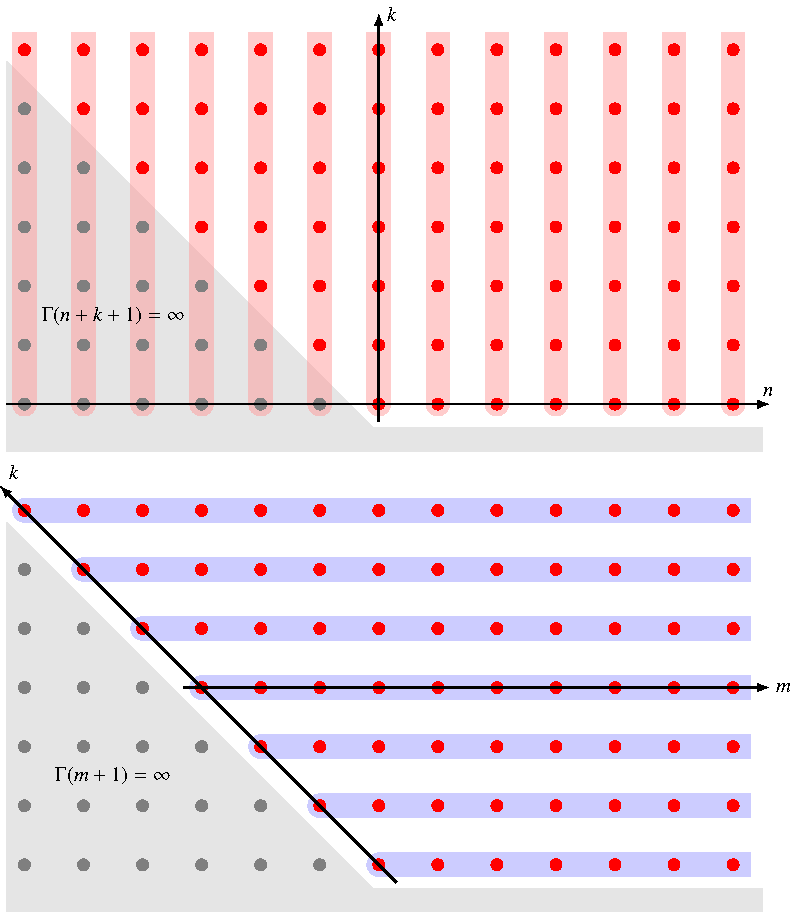
\includegraphics{chapters/050-differential/images/besselgrid.pdf}
\caption{Indexmenge für Herleitung der erzeugenden Funktion der
Besselfunktionen.
Die rote Summe in \eqref{buch:differentialgleichungen:bessel:eqn:rotesumme}
entspricht den vertikalen roten Streifen oben,
die blaue Summe in
\eqref{buch:differentialgleichungen:bessel:eqn:blauesumme}
den horizontalen Streifen in der Abbildung unten.
Alle Terme enthalten $\Gamma(n+k+1)$ im Nenner,
im grau hinterlegten Gebiet verschwinden sie.
\label{buch:differentialgleichungen:bessel:fig:indexmenge}}
\end{figure}
Die erzeugende Funktion der Bessel-Funktionen ist die Summe
\begin{align}
\sum_{n\in\mathbb{Z}} J_n(x)z^n
&=
\sum_{n\in\mathbb{Z}}
{\color{darkred}
\sum_{k=0}^\infty
\frac{(-1)^k}{k!\,\Gamma(k+n+1)}
\biggl(\frac{x}{2}\biggr)^{2k+n}
}
z^n.
\label{buch:differentialgleichungen:bessel:eqn:rotesumme}
\intertext{Die rote Summe entspricht den vertikalen roten Streifen in
Abbildung~\ref{buch:differentialgleichungen:bessel:fig:indexmenge} oben.
Die grau hinterlegten Punkte in der Abbildung gehören zu verschwindenden
Termen.
Wir schreiben $m=k+n$ und drücken alle Terme durch $k$ und $m$ aus:}
&=
\sum_{n\in \mathbb{Z}}
\sum_{k=0}^\infty
\frac{(-1)^k}{k!\,\Gamma(n+k+1)}
\biggl(\frac{x}{2}\biggr)^k
\biggl(\frac{x}{2}\biggr)^{n+k}
z^{n+k}
z^{-k}
\notag
\\
&=
\sum_{m\in \mathbb{Z}}
\sum_{k=0}^\infty \frac{(-1)^k}{k!}
\biggl(\frac{x}{2}\biggr)^k
z^{-k}
\frac{1}{\Gamma(m+1)}
\biggl(\frac{x}{2}\biggr)^{m}
z^{n+k}
\notag
\intertext{Auch in dieser Summe fallen wieder die Terme mit $m<0$
wegen $\Gamma(m+1)=\infty$ weg.
Die Grenzen der Summation über $k$ hängen nicht von $m$ ab, daher
können wir die Summationsreihenfolge vertauschen.
Die Summation über $m$ entspricht den horizontalen blauen Streifen
in 
Abbildung~\ref{buch:differentialgleichungen:bessel:fig:indexmenge}
unten.
Es ergibt sich die Summe}
&=
\sum_{k=0}^\infty
\sum_{m=0}^\infty
\frac{(-1)^k}{k!}
\biggl(\frac{x}{2}\biggr)^k
z^{-k}
\frac{1}{\Gamma(m+1)}
\biggl(\frac{x}{2}\biggr)^{m}
z^{m}
\notag
\\
&=
\sum_{k=0}^\infty \frac{(-1)^k}{k!}
\biggl(\frac{x}{2}\biggr)^k
z^{-k}
\cdot
{\color{blue}
\sum_{m=0}^\infty
\frac{1}{\Gamma(m+1)}
\biggl(\frac{x}{2}\biggr)^{m}
z^{m}
}.
\label{buch:differentialgleichungen:bessel:eqn:blauesumme}
\intertext{Beide Reihen sind Exponentialreihen, was man besser sehen kann,
wenn man die Gamma-Funktion in der zweiten Summe wieder als die
Fakultät $\Gamma(m+1)=m!$ schreibt.
Die beiden Exponentialreihen sind
}
&=
\sum_{k=0}^\infty \frac{\bigl(-\frac{x}2\cdot\frac1z\bigr)}{k!}
\cdot
\sum_{m=0}^\infty
\frac{\bigl(z\frac{x}2\bigr)^m}{m!}
=
\exp\biggl(\frac{x}2\cdot\biggl(-\frac1z\biggr)\biggr)
\cdot
\exp\biggl(\frac{x}2\cdot z\biggr)
=
\exp\biggl(\frac{x}2\cdot\biggl(z-\frac1z\biggr)\biggr).
\notag
\end{align}

%
% Additionstheorem
%
\subsubsection{Additionstheorem}
Die erzeugende Funktion kann dazu verwendet werden, das Additionstheorem
für die Besselfunktionen zu beweisen.

\begin{satz}
Für $l\in\mathbb{Z}$ und $x,y\in\mathbb{R}$ gilt
\[
J_l(x+y) = \sum_{m=-\infty}^\infty J_m(x)J_{l-m}(y).
\]
\end{satz}

\begin{proof}[Beweis]
Die Koeffizienten der erzeugenden Funktion der Bessel-Funktionen für
das Argument $x+y$ ist
\begin{align*}
\exp\biggl(\frac{x+y}2\biggl(z+\frac1z\biggr)\biggr)
&=
\sum_{n=-\infty}^\infty J_n(x+y)z^n.
\intertext{%
Wir verwenden die Exponentialgesetze auf der linken Seite und 
erhalten}
&=
\exp\biggl(\frac{x}2\biggl(z+\frac1z\biggr)\biggr)
\cdot
\exp\biggl(\frac{y}2\biggl(z+\frac1z\biggr)\biggr).
\intertext{Beide Faktoren sind erzeugende Funktionen von Bessel-Funktionen,
wir können sie also als}
&=
\sum_{m=-\infty}^\infty J_m(x)z^m
\cdot
\sum_{k=-\infty}^\infty J_k(y)z^k
\intertext{schreiben.
Durch Ausmultiplizieren und Zusammenfassen von Termen mit gleichem
Exponenten finden wir
}
&=
\sum_{m,k} J_m(x)J_k(y) z^{k+m}
=
\sum_{l=-\infty}^\infty
\biggl(
\sum_{m=-\infty}^\infty J_m(x)J_{l-m}(y)
\biggr)
z^l.
\intertext{Daraus folgt schliesslich mit Koeffizientenvergleich das
Additionstheorem}
J_l(x+y) &= \sum_{m=-\infty}^\infty J_m(x)J_{l-m}(y)
\end{align*}
für alle $l$.
\end{proof}

%
% Der Fall \alpha=0
% 
\subsubsection{Der Fall $\alpha=0$}
Im Fall $\alpha=0$ hat das Indexpolynom eine doppelte Nullstelle, wir
können daher nur eine Lösung erwarten.
Im Fall $\alpha=0$ wird das Produkt im Nenner zu $n!$, so dass die
Lösungsfunktion
\[
J_0(x)
=
\sum_{k=0}^\infty
\frac{(-1)^k}{(k!)^2}
\biggl(\frac{x}{2}\biggr)^{2k}
\]
geschrieben werden kann.


%
% Der Fall \alpha=p, p\in \mathbb{N}
%
\subsubsection{Der Fall $\alpha=p$, $p\in\mathbb{N}, p > 0$}
In diesem Fall kann nur die erste
Lösung~\eqref{buch:differentialgleichunge:bessel:erste}
verwendet werden.
Damit erhält die Lösungsfunktion die Form
\[
J_p(x)
=
\sum_{k=0}^\infty
\frac{(-1)^k}{k!(p+k)!}\biggl(\frac{x}{2}\biggr)^{p+2k}.
\]

%
% Der Fall $\alpha=n+\frac12$
%
\subsubsection{Der Fall $\alpha=n+\frac12$, $n\in\mathbb{N}$}
Obwohl $2\alpha$ eine Ganzzahl ist, sind die beiden Lösungen
\label{buch:differentialgleichunge:bessel:erste}
und
\label{buch:differentialgleichunge:bessel:zweite}
linear unabhängig.

Man kann zeigen, dass sich die Lösungsfunktionen in diesem Fall
durch bereits bekannte elementare Funktionen ausdrücken lassen.
Wir rechnen dies für $n=0$ nach.
Zunächst drücken wir die Pochhammer-Symbole im Nenner anders aus.
Es ist
\begin{align*}
\biggl(\frac12 + 1\biggr)_k
&=
\biggl(\frac12 + 1\biggr)
\biggl(\frac12 + 2\biggr)
\cdots
\biggl(\frac12 + k\biggr)
=
\frac{1}{2^k}\bigl(3\cdot 5\cdot\ldots\cdot (2k+1)\bigr)
=
\frac{(2k+1)!}{2^{2k}\cdot k!}
\\
\biggl(-\frac12 + 1\biggr)_k
&=
\biggl(-\frac12 + 1\biggr)
\biggl(-\frac12 + 2\biggr)
\cdots
\biggl(-\frac12 + k\biggr)
\\
&=
\biggl(\frac12 + 0\biggr)
\biggl(\frac12 + 1\biggr)
\cdots
\biggl(\frac12 + k-1\biggr)
=
\frac{1}{2^k}\bigl(1\cdot 3 \cdot\ldots\cdot (2(k-1)+1)\bigr)
=
\frac{(2k-1)!}{2^{2k-1}\cdot (k-1)!}
\end{align*}
Damit können jetzt die Reihenentwicklungen der Lösung wie folgt
umgeformt werden
\begin{align*}
y_1(x)
&=
x^\alpha
\sum_{k=0}^\infty
\frac{1}{(\alpha+1)_k}
\frac{(-x^2/4)^k}{k!}
=
\sqrt{x}
\sum_{k=0}^\infty
\frac{2^{2k}k!}{(2k+1)!}
\frac{(-x^2/4)^k}{k!}
=
\sqrt{x}
\sum_{k=0}^\infty
(-1)^k
\frac{x^{2k}}{(2k+1)!}
\\
&=
\frac{1}{\sqrt{x}}
\sum_{k=0}^\infty
(-1)^k
\frac{x^{2k+1}}{(2k+1)!}
=
\frac{1}{\sqrt{x}} \sin x
\\
y_2(x)
&=
x^{-\alpha}
\sum_{k=0}^\infty
\frac{1}{(-\alpha+1)_k}
\frac{(-x^2/4)^k}{k!}
=
x^{-\frac12}
\sum_{k=0}^\infty
\frac{2^{2k-1}\cdot (k-1)!}{(2k-1)!}
\frac{(-x^2/4)^k}{k!}
\\
&=
\frac{1}{\sqrt{x}}
\sum_{k=0}^\infty
(-1)^k
\frac{x^{2k}}{(2k-1)!\cdot 2k}
=
\frac{1}{\sqrt{x}} \cos x.
\end{align*}

Die Bessel-Funktionen verwenden aber eine andere Normierung. 
Die Gleichung~\eqref{buch:differentialgleichungen:bessel:normierungsgleichung}
zeigt, dass die Bessel-Funktionen durch Division
der Funktion $y_1(x)$ und $y_2(x)$ durch $2^\alpha \Gamma(\alpha+1)$ 
erhalten werden können.
Dies ergibt
\begin{equation*}
\renewcommand{\arraycolsep}{1pt}
\begin{array}{rclclclcl}
J_{\frac12}(x)
&=&
\displaystyle\frac{1}{2^{\frac12}\Gamma(\frac12+1)}
y_1(x)
&=&
\displaystyle\frac{1}{2^{\frac12}\frac12\Gamma(\frac12)}
y_1(x)
&=&
\displaystyle\frac{\sqrt{2}}{\Gamma(\frac12)}
y_1(x)
&=&
\displaystyle\frac{1}{\Gamma(\frac12)}
\sqrt{ \frac{2}{x}}
\sin x,
\\
J_{-\frac12}(x)
&=&
\displaystyle\frac{1}{2^{-\frac12}\Gamma(-\frac12+1)}
y_2(x)
&=&
\displaystyle\frac{2^{\frac12}}{\Gamma(\frac12)}
y_2(x)
&=&
\displaystyle\frac{\sqrt{2}}{\Gamma(\frac12)}
y_2(x)
&=&
\displaystyle\frac{1}{\Gamma(\frac12)}
\sqrt{\frac{2}{x}}
\cos x.
\end{array}
\end{equation*}
Wegen $\Gamma(\frac12)=\sqrt{\pi}$ sind die
halbzahligen Bessel-Funktionen daher
\begin{align*}
J_{\frac12}(x)
&=
\sqrt{\frac{2}{\pi x}} \sin x
=
\sqrt{\frac{2}{\pi}} x^{-\frac12}\sin x
&
&\text{und}&
J_{-\frac12}(x)
&=
\sqrt{\frac{2}{\pi x}} \cos x
=
\sqrt{\frac{2}{\pi}} x^{-\frac12}\cos x.
\end{align*}

%
% Direkte Verifikation der Lösungen
%
\subsubsection{Direkte Verifikation der Lösungen für $\alpha=\pm\frac12$}
Tatsächlich führt die Anwendung des Bessel-Operators auf die beiden
Funktionen auf
\begin{align*}
\sqrt{\frac{\pi}2}
BJ_{\frac12}(x)
&=
\sqrt{\frac{\pi}2}
\biggl(
x^2J_{\frac12}''(x) + xJ_{\frac12}'(x) + x^2J_{\frac12}(x)
\biggr)
\\
&=
x^2(x^{-\frac12}\sin x)''
+
x(x^{-\frac12}\sin x)'
+
x^2(x^{-\frac12}\sin x)
\\
&=
x^2(
x^{-{\textstyle\frac12}}\cos x
-{\textstyle\frac12}x^{-\frac32}\sin x
)'
+
x(
x^{-\frac12}\cos x
-{\textstyle\frac12}x^{-\frac32}\sin x
)
+
x^{\frac32}\sin x
\\
&=
x^2(
-x^{-\frac12}\sin x
-{\textstyle\frac12}x^{-\frac32}\cos x
-{\textstyle\frac12}x^{-\frac32}\cos x
+{\textstyle\frac{3}{4}}x^{-\frac52}\sin x
)
+
x^{\frac12}\cos x
+
x^{-\frac12}(x-{\textstyle\frac12})\sin x
\\
&=
(
-x^{\frac32}
+{\textstyle\frac34}x^{-\frac12}
+x^{\frac32}
-{\textstyle\frac12}x^{-\frac12}
)
\sin x
=
\frac14x^{-\frac12}\sin x
=
\frac14
\sqrt{\frac{\pi}2}
J_{\frac12}(x)
\\
BJ_{\frac12}(x)
&=
\biggl(\frac12\biggr)^2 J_{\frac12}(x).
\end{align*}
Dies zeigt, dass $J_{\frac12}(x)$ tatsächlich eine Eigenfunktion
des Bessel-Operators zum Eigenwert $\alpha^2 = \frac14$ ist.
Analog kann man die Lösung $y_2(x)$ für $-\frac12$ verifizieren.


%
% hypergeometrisch.tex
%
% (c) 2021 Prof Dr Andreas Müller, OST Ostschweizer Fachhochschule
%
\section{Hypergeometrische Funktionen
\label{buch:rekursion:section:hypergeometrische-funktion}}
\rhead{Hypergeometrische Funktionen}
Kann man eine Formel für die Lösung $S_n$ der lineare Differenzengleichung
\[
n^3S_{n}
=
16(n-{\textstyle\frac12})(2n^2-2n+1)S_{n-1}
-256(n-1)^3S_3
\]
mit Anfangswerten $S_0=1$ und $S_1=8$ angeben?
Dies scheint auf den ersten Blick unmöglich kompliziert, man kann aber
zeigen, dass
\[
S_n
=
\sum_{k=0}^n 
\binom{2n-2k}{n-k}^2 \binom{2k}{k}^2
\]
gilt (\cite[p.~xi]{buch:ab}).
Die Lösung ist also eine Summe von Summanden, die sehr viel einfacher
aussehen und vor allem die besondere Eigenschaft haben, dass die
Quotienten aufeinanderfolgender Terme rationale Funktionen von von $k$
sind.
% XXX Quotient berechnen

Eine besonders simple solche Funktion ist die geometrische Reihe, die
im Abschnitt~\ref{buch:rekursion:hypergeometrisch:geometrisch}
in Erinnerung gerufen wird.
Abschnitt~\ref{buch:rekursion:hypergeometrisch:reihen}
definiert den Begriff der hypergeometrischen Reihe und zeigt, 
wie sie in eine Standardform gebracht werden können.
In Abschnitt~\ref{buch:rekursion:hypergeometrisch:beispiele}
schliesslich wird an Hand von Beispielen gezeigt, wie bekannte
Funktionen als hypergeometrische Funktionen interpretiert werden können.

\subsection{Die geometrische Reihe
\label{buch:rekursion:hypergeometrisch:geometrisch}}
Die besonders einfache Potenzreihe
\[
f(q)
=
\sum_{k=0}^\infty aq^k
\]
heisst die {\em geometrische Reihe}.
Die Partialsummen 
\[
S_n
=
\sum_{k=0}^n aq^k
\]
kann mit der Differenz
\begin{equation}
(1-q)S_n
=
S_n - qS_n
=
\sum_{k=0}^n aq^k
-
\sum_{k=1}^{n+1} aq^k
=
a -aq^{n+1}
\label{buch:rekursion:hypergeometrisch:eqn:qsumme}
\end{equation}
berechnet werden, die man nach
\begin{equation}
S_n 
=
a\frac{1-q^{n+1}}{1-q}
\label{buch:rekursion:hypergeometrisch:eqn:geomsumme}
\end{equation}
auflösen kann.

Fü $q<1$ geht $q^n\to 0$ und damit konvergiert
$S_n$  gegen
\[
\sum_{k=0}^\infty aq^k
=
a\frac{1}{1-q}.
\]

Die geometrische Reihe ist charakterisiert dadurch, dass aufeinanderfolgende
Terme den gleichen Quotienten
\[
\frac{aq^{k+1}}{aq^k}
=
q
\]
haben.
Die Berechnung der Summe in 
\eqref{buch:rekursion:hypergeometrisch:eqn:qsumme}
beruht darauf, dass die Multiplikation mit $q$ einen ``anderen''
Teil der Summe ergibt, der sich in der Differenze weghebt.

\subsection{Hypergeometrische Reihen
\label{buch:rekursion:hypergeometrisch:reihen}}
Es ist plausibel, dass eine etwas lockerere Bedingung an die
Quotienten aufeinanderfolgender Terme einer Reihe immer noch
ermöglichen wird, interessante Aussagen über die durch die
Reihe beschriebenen Funktionen zu machen.

\begin{definition}
Eine Reihe
\[
f(x) = \sum_{k=0}^\infty a_k x^k
\]
heisst {\em hypergeometrisch}, wenn der Quotient aufeinanderfolgender
Koeffizienten eine rationale Funktion von $k$ ist,
wenn also
\[
\frac{a_{k+1}}{a_k}
=
\frac{p(k)}{q(k)}
\]
mit Polynomen $p(k)$ und $q(k)$ ist.
\end{definition}

Die geometrische Reihe ist natürlich eine hypergeometrische Reihe,
wobei $p(k)/q(k)=1$ ist.
Etwas interessanter ist die Exponentialfunktion, durch die Taylor-Reihe
\[
e^x = \sum_{k=0}^\infty \frac{x^k}{k!}
\]
dargestellt werden kann.
Der Quotient aufeinanderfolgender Koeffizienten ist
\[
\frac{a_{k+1}}{a_k}
=
\frac{1/(k+1)!}{1/k!}
=
\frac{k!}{(k+1)!}
=
\frac{1}{k+1},
\]
eine rationale Funktion mit Zählergrad $0$ und Nennergrad $1$.

Die Kosinus-Funktion wird durch die Taylor-Reihe
\[
\cos x = \sum_{k=0}^\infty \frac{(-1)^k}{(2k)!} x^{2k}
\]
dargestellt.
Als Potenzreihe in $x$ kann die Kosinus-Reihe nicht hypergeometrisch sein,
die ungeraden Koeffizienten verschwinden und damit undefinierte
Quotienten haben.
Als Reihe in $z=x^2$ ist aber
\[
\sum_{k=0}^\infty \frac{(-1)^k}{(2k)!} z^k
\qquad\Rightarrow\qquad
a_k = \frac{(-1)^k}{(2k)!}
\]
hypergeometrisch, weil der Quotient aufeinanderfolgender Koeffizienten
\[
\frac{a_{k+1}}{a_k}
=
\frac{(-1)^{k+1}}{(2k+2)!}\cdot \frac{(2k)!}{(-1)^k}
=
-\frac{1}{(2k+2)(2k+1)},
\]
eine rationale Funktion mit Zählergrad $0$ und Nennergrad $2$.
Es gibt also eine hypergeometrische Reihe $f(z)$ derart, dass
$\cos x = f(x^2)$ ist.

Seien $p(k)$ und $q(k)$ zwei Polynome derart, dass
\[
\frac{a_{k+1}}{a_k} = \frac{p(k)}{q(k)}.
\]
Daraus lässt sich der Koeffizient $a_{k+1}$ als
\begin{equation}
a_{k+1}
=
\frac{p(k)}{q(k)}
\cdot
a_k
=
\frac{p(k)}{q(k)}
\cdot
\frac{p(k-1)}{q(k-1)}
\cdot
a_{k-1}
=\dots=
\frac{p(k)}{q(k)}
\frac{p(k-1)}{q(k-1)}
\cdots
\frac{p(1)}{q(1)}
\frac{p(0)}{q(0)}
a_0
\label{buch:rekursion:hypergeometrisch:ak+1}
\end{equation}
berechnen.
Alle Koeffizienten haben also den Faktor $a_0=f(0)$ gemeinsam.

Die Produkte von Quotienten $p(k)/q(k)$ sollen jetzt weiter
vereinfacht werden.
Sei $n$ der Grad von $p(k)$ und $m$ der Grad von $q(k)$.
Dazu nehmen wir an, dass $a_i$, $i=1,\dots,n$ die Nullstellen von $p(k)$ sind
und $b_j$, $j=1,\dots,m$ die Nullstellen von $q(k)$, dass man also
die Polynome als
\begin{align*}
p(k) &= x(k-a_1)(k-a_2)\cdots(k-a_n)
\\
q(k) &= (k-b_1)(k-b_2)\cdots(k-b_m)
\end{align*}
schreiben kann.
Der Faktor $x$ ist nötig, weil die Polynome $p(k)$ und $q(k)$ nicht
notwendigerweise normiert sind.

Um das Produkt der Quotienten zu vereinfachen, nehmen wir für den Moment
an, dass Zähler und Nenner vom Grad $n=m=1$ ist.
Dann ist nach 
\eqref{buch:rekursion:hypergeometrisch:ak+1}
\[
a_{k}
=
x^{k}
\frac{
(k-1-a_1) \cdots (2-a_1)(1-a_1)(0-a_1)
}{
(k-1-b_1) \cdots (2-b_1)(1-b_1)(0-b_1)
}
=
\frac{(-a_1)_k}{(-b_1)_k} x^k.
\]
Die Koeffizienten können daher als Quotienten von Pochhammer-Symbolen
geschrieben werden.
Für Polynome $p(k)$ und $q(k)$ höheren Grades sind die Koeffizienten
von der Form
\[
a_k
=
\frac{(-a_1)_k(-a_2)_k\cdots (-a_n)_k}{(-b_1)_k(-b_2)_k\cdots(-b_m)_k}
x^ka_0.
\]
Jede hypergeometrische Reihe kann daher in der Form
\[
a_0
\sum_{k=0}^\infty
\frac{(-a_1)_k(-a_2)_k\cdots (-a_n)_k}{(-b_1)_k(-b_2)_k\cdots(-b_m)_k}
x^k
\]
geschrieben werden.

\begin{definition}
\label{buch:rekursion:hypergeometrisch:def}
Die hypergeometrische Funktion
$\mathstrut_pF_q$ ist definiert durch die Reihe
\[
\mathstrut_pF_q
\biggl(
\begin{matrix}
a_1,\dots,a_p\\
b_1,\dots,b_q
\end{matrix}
;
x
\biggr)
=
\mathstrut_pF_q(a_1,\dots,a_p;b_1,\dots,b_q;x)
=
\sum_{k=0}^\infty
\frac{(a_1)_k\cdots(a_p)_k}{(b_1)_k\cdots(b_q)_k}\frac{x^k}{k!}.
\]
\end{definition}

Da $(1)_k=k!$ hätte die Definition den Nenner $k!$ in der Reihe
auch durch eines der Pochhammer-Symbole ausdrücken können.
Wird dieser Nenner nicht gebraucht, kann man ihn durch einen 
zusätzlichen Faktor $(1)_k$ im Zähler des Bruchs von Pochhammer-Symbolen
kompensieren, wodurch sich der Grad $p$ des Zählers natürlich um $1$
erhöht.

Die oben analysierte Summe $S$ kann mit der Definition als
\[
S
=
a_0
\,
\mathstrut_{n+1}F_m \biggl(
\begin{matrix}
-a_1,-a_2,\dots,-a_n,1\\
-b_1,-b_2,\dots,-a_m
\end{matrix}; x
\biggr)
\]
beschrieben werden.

\subsection{Beispiele von hypergeometrischen Funktionen
\label{buch:rekursion:hypergeometrisch:beispiele}}
Viele der bekannten Reihenentwicklungen häufig verwendeter Funktionen
lassen sich durch die hypergeometrischen Funktionen von
Definition~\ref{buch:rekursion:hypergeometrisch:def} ausdrücken.
In diesem Abschnitt werden einige Beispiel dazu gegeben.

\subsubsection{Die geometrische Reihe}
In der geometrischen Reihe fehlt der Nenner $k!$, es braucht
daher einen Term $(1)_k$ im Zähler, um den Nenner zu kompensieren.
Somit ist die geometrische Reihe
\[
\frac{a}{1-x}
=
\sum_{k=0}^\infty
ax^k
=
a\sum_{k=0}^\infty
\frac{(1)_k}{1}
\frac{x^k}{k!}
=
a\,\mathstrut_1F_0(1,x).
\]

\subsubsection{Exponentialfunktion}
Die Exponentialfunktion ist die Reihe
\[
e^x = \sum_{k=0}^\infty \frac{x^k}{k!}.
\]
In diesem Fall werden keine Quotienten von Pochhammer-Symbolen
benötigt, es ist daher
\[
e^x = \mathstrut_0F_0(x).
\]

\subsubsection{Wurzelfunktion}
Die Wurzelfunktion $x\mapsto \sqrt{x}$ hat keine Taylor-Entwicklung
in $x=0$, aber die Funktion $x\mapsto\sqrt{1+x}$ hat die Taylor-Reihe
\[
\sqrt{1+x}
=
1
+
\frac12 x
-
\frac{1\cdot 1}{2\cdot 4}x^2
+
\frac{1\cdot 1\cdot 3}{2\cdot 4\cdot 6}x^3
-
\frac{1\cdot 1\cdot 3\cdot 5}{2\cdot 4\cdot 6\cdot 8}x^4
+
\dots
\]
Um die Verbindung zu einer hypergeometrischen Funktion herzustellen,
müssen wir den Term $x^k/k!$ abspalten.
Dann wird
\begin{align*}
\sqrt{1+x}
&=
1
+
\frac12 \frac{x}{1!}
-
\frac{1\cdot 1}{2^2}\frac{x^2}{2!}
+
\frac{1\cdot 1\cdot 3}{2^3}\frac{x^3}{3!}
-
\frac{1\cdot 1\cdot 3\cdot 5}{2^4}\frac{x^4}{4!}
+
\dots
\\
&=
1
+
\frac12 \cdot\frac{x}{1!}
-
\frac{1}{2}\cdot \frac{1}{2}\cdot\frac{x^2}{2!}
+
\frac{1}{2}\cdot \frac{1}2\cdot \frac{3}{2}\cdot\frac{x^3}{3!}
-
\frac{1}{2}\cdot \frac{1}{2}\cdot \frac{3}{2}\cdot \frac{5}{2}\cdot\frac{x^4}{4!}
+
\dots
\end{align*}
Es ist noch etwas undurchsichtig, warum die ersten beiden Terme
das gleiche Vorzeichen haben und warum der Faktor $\frac12$ in jedem
Term zweimal vorkommt.
Diese Unklarheit kann jedoch beseitigt werden, wenn man den ersten
Faktor als $-\frac12$ schreibt:
\begin{align*}
\sqrt{1+x}
&=
1
-
\biggl(-\frac12\biggr)\cdot\frac{x}{1!}
+
\biggl(-\frac{1}{2}\biggr)\cdot \frac{1}{2}\cdot\frac{x^2}{2!}
-
\biggl(-\frac{1}{2}\biggr)\cdot \frac{1}2\cdot \frac{3}{2}\cdot\frac{x^3}{3!}
+
\biggl(-\frac{1}{2}\biggr)\cdot \frac{1}{2}\cdot \frac{3}{2}\cdot \frac{5}{2}\cdot\frac{x^4}{4!}
+
\dots
\\
&=
1 + 
\biggl(-\frac12\biggr)\cdot\frac{-x}{1!}
+
\biggl(-\frac{1}{2}\biggr)\cdot \frac{1}{2}\cdot\frac{(-x)^2}{2!}
+
\biggl(-\frac{1}{2}\biggr)\cdot \frac{1}2\cdot \frac{3}{2}\cdot\frac{(-x)^3}{3!}
+
\biggl(-\frac{1}{2}\biggr)\cdot \frac{1}{2}\cdot \frac{3}{2}\cdot \frac{5}{2}\cdot\frac{(-x)^4}{4!}
+
\dots
\end{align*}
Die Koeffizienten sind aufsteigende Produkte mit $k$ Faktoren, die alle bei
$-\frac12$ beginnen, sie können daher als Pochhammer-Symbole $(-\frac12)_k$
geschrieben werden.
Die Wurzelfunktion ist daher die hypergeometrische Funktion
\[
\sqrt{1\pm x}
=
\sum_{k=0}^\infty
\biggl(-\frac12\biggr)_k \frac{(-x)^k}{k!}
=
\mathstrut_1F_0(-{\textstyle\frac12};\mp x).
\]

\subsubsection{Logarithmusfunktion}
Für $x\in (-1,1)$ konvergiert die Taylor-Reihe
\[
\log(1+x)
=
x-\frac{x^2}{2}+\frac{x^3}{3}-\frac{x^4}{4}+\dots
\]
der Logarithmusfunktion im Punkt $x=0$.
Die Reihe beginnt nicht mit einem konstanten Term, daher klammern wir
zunächst einen Faktor $x$ aus:
\[
\log(1+x)
=
x\cdot
\biggl(
1-\frac{x}{2}+\frac{x^2}{3}-\frac{x^3}{4}+\dots
\biggr)
\]
Um dies in die Form einer hypergeometrischen Funktion zu bringen,
muss zunächst wieder der Nenner $k!$ hergestellt werden.
\begin{align*}
\log(1+x)
&=
x\cdot\biggl(
1
- \frac{1!}{2} \frac{x}{1!}
+ \frac{2!}{3} \frac{x^2}{2!} 
- \frac{3!}{4} \frac{x^3}{3!}+\dots
\biggr).
\intertext{Den Nenner $k+1$ kann man als Quotienten $k!/(k+1)!$ erhalten,
also}
\log(1+x)
&=
x\cdot\biggl(
1
- \frac{(1!)^2}{2!} \frac{x}{1!}
+ \frac{(2!)^2}{3!} \frac{x^2}{2!} 
- \frac{(3!)^2}{4!} \frac{x^3}{3!}+\dots
\biggr).
\end{align*}
Die Fakultät
\[
(k+1)!
=
1\cdot 2 \cdot 3 \cdot\ldots\cdot k\cdot (k+1)
=
2 \cdot (2 + 1) \cdot (2+2) \cdot\ldots\cdot (2+k-2) \cdot (2+k-1)
=
(2)_{k}
\]
ist auch ein Pochhammer-Symbol, so dass die Logarithmusfunktion
zur hypergeometrischen Funktion
\[
\log(1+x)
=
x\cdot\biggl(
1
+ \frac{(1)_1(1)_1}{(2)_1} \frac{(-x)}{1!}
+ \frac{(1)_2(1)_2}{(2)_2} \frac{(-x)^2}{2!} 
+ \frac{(1)_3(1)_3}{(2)_2} \frac{(-x)^3}{3!}+\dots
\biggr)
=
x\cdot
\mathstrut_2F_1\biggl(\begin{matrix}1,1\\2\end{matrix};-x\biggr).
\]


\subsubsection{Trigonometrische Funktionen}
Die Kosinus-Funktion wurde bereits als hypergeometrische Funktion erkannt,
im Folgenden soll dies auch noch für die Sinus-Funktion
durchgeführt werden.
Die Taylor-Reihe der Sinus-Funktion im Punkt $0$ ist
\begin{align*}
\sin x
&=
x-\frac{x^3}{3!}+\frac{x^5}{5!}-\frac{x^7}{7!}+\dots
\end{align*}
In dieser Reihe fehlen die geraden Potenzen, wir Klammern daher einen
Faktor $x$ aus und schreiben den Rest als eine Funktion von $-x^2$
\begin{align*}
\sin x
&=
x
\biggl(
1+\frac{-x^2}{3!}+\frac{(-x^2)^2}{5!}-\frac{(-x^2)^3}{7!}+\dots
\biggr)
=
x f(-x^2).
\end{align*}
Die Funktion $f(z)$ soll jetzt als hypergeometrische Funktion geschrieben
werden.
Dazu muss zunächst wieder der Nenner $k!$ wiederhergestellt werden:
\[
f(z)
=
1
+
\frac{1!}{3!}\cdot \frac{z}{1!}
+
\frac{2!}{5!}\cdot \frac{z^2}{2!}
+
\frac{3!}{7!}\cdot \frac{z^3}{3!}
+
\dots
\]
Die Koeffizienten $k!/(2k+1)!$ müssen jetzt durch Pochhammer-Symbole
mit jeweils $k$ Faktoren ausgedrückt werden.
Dazu muss die Fakultät $(2k+1)!$ in zwei Produkte
\[
(2k+1)
=
2\cdot 3 \cdot 4\cdot 5\cdot \ldots \cdot 2k \cdot (2k+1)
=
(2\cdot 4 \cdot 6\cdot\ldots\cdot 2k)
\cdot
(3\cdot 5\cdot 7\cdot \ldots \cdot (2k+1))
\]
aufgespaltet werden.
Diese Produkte haben zwar $k$-Faktoren, aber sie sind keine
Pochhammer-Symbole, weil die Differenz aufeinanderfolgender Faktoren 
jeweils $2$ ist.
Wir dividieren die geraden Faktoren durch $2$ und dividieren die 
ungeraden durch $2$, dadurch ändert sich das Produkt nicht und wird
\[
(2k+1)!
=
(1\cdot2\cdot3\cdot\ldots\cdot k)
\cdot
\biggl(
\frac{3}{2}\cdot
\frac{5}{2}\cdot
\frac{7}{2}\cdot
\ldots\cdot
\frac{2k+1}{2}
\biggr)
=
(1)_k\cdot \biggl(\frac{3}{2}\biggr)_k
\]
Setzt man dies in die Reihe ein, wird
\[
f(z)
=
\sum_{k=0}^\infty
\frac{(1)_k}{(1)_k\cdot (\frac{3}{2})_k}
z^k
=
\mathstrut_1F_2(1;1,\frac{3}{2};z).
\]
Damit lässt sich die Sinus-Funktion als
\begin{equation}
\sin x
=
x\,\mathstrut_1F_2\biggl(\begin{matrix}1\\1,\frac32\end{matrix};-x^2\biggr)
=
x\,\mathstrut_1F_2\biggl(\begin{matrix}\text{---}\\\frac32\end{matrix};-x^2\biggr)
\label{buch:rekursion:hypergeometrisch:eqn:sinhyper}
\end{equation}
durch eine hypergeometrische Funktion ausdrücken.

\subsubsection{Hyperbolische Funktionen}
Die für die Sinus-Funktion angewendete Methode lässt sich auch
auf die Funktion 
\begin{align*}
\sinh x
&=
\sum_{k=0}^\infty \frac{x^{2k+1}}{(2k+1)!}
\\
&=
x
\,
\biggl(
1+\frac{x^2}{3!} + \frac{x^4}{5!}+\frac{x^6}{7!}+\dots
\biggr)
\\
&=
xf(-x^2)
=
x\,\mathstrut_1F_2\biggl(
\begin{matrix}1\\1,\frac{3}{2}\end{matrix}
;x^2
\biggr)
=
x\,\mathstrut_0F_1\biggl(
\begin{matrix}\text{---}\\,\frac{3}{2}\end{matrix}
;x^2
\biggr).
\end{align*}
Bis auf das Vorzeichen des Arguments der hypergeometrischen Funktion
ist diese Darstellung identisch mit der von $\sin x$.
Dies illustriert die Rolle der hypergeometrischen Funktionen als
``grosse Vereinheitlichung'' der bekannten speziellen Funktionen.

%
% Ableitung und Stammfunktion
%
\subsection{Ableitung und Stammfunktion hypergeometrischer Funktionen}
Sowohl Ableitung wie auch Stammfunktion einer hypergeometrischen
Funktion lässt sich immer durch hypergeometrische Reihen ausdrücken.

\subsubsection{Ableitung}
Wir gehen aus von der Funktion
\begin{equation}
f(x)
=
\mathstrut_nF_m\biggl(
\begin{matrix}a_1,\dots,a_n\\b_1,\dots,b_m\end{matrix};
x\biggr)
=
\sum_{k=0}^\infty
\frac{
(a_1)_k\cdot\ldots\cdot(a_n)_k
}{
(b_1)_k\cdot\ldots\cdot(b_m)_k
}
\frac{x^k}{k!}.
\label{buch:rekursion:hypergeometrisch:eqn:f}
\end{equation}
Die Ableitung von $f(x)$ ist
\[
f'(x)
=
\sum_{k=0}^\infty
\frac{
(a_1)_k\cdot\ldots\cdot(a_n)_k
}{
(b_1)_k\cdot\ldots\cdot(b_m)_k
}
\frac{x^{k-1}}{(k-1)!}
=
\sum_{k=1}^\infty
\frac{
(a_1)_{k+1}\cdot\ldots\cdot(a_n)_{k+1}
}{
(b_1)_{k+1}\cdot\ldots\cdot(b_m)_{k+1}
}
\frac{x^k}{k!}.
\]
Der Koeffizient besteht zwar aus lauter Pochhammer-Symbolen, aber sie
haben jeweils zu einen Faktor zuviel.
Indem man den jeweils ersten Faktor ausklammert, kann man die
Terme wieder in die Form einer hypergeometrischen Reihe bringen.
\begin{align*}
f'(x)
&=
\sum_{k=1}^\infty
\frac{
a_1(a_1)_{k}\cdot\ldots\cdot a_n(a_n)_{k}
}{
b_1(b_1)_{k}\cdot\ldots\cdot b_m(b_m)_{k}
}
\frac{x^k}{k!}
\\
&=
\sum_{k=1}^\infty
\frac{
a_1\cdot\ldots\cdot a_n
}{
b_1\cdot\ldots\cdot b_m
}
\frac{
(a_1+1)_{k}\cdot\ldots\cdot(a_n+1)_{k}
}{
(b_1+1)_{k}\cdot\ldots\cdot(b_m+1)_{k}
}
\frac{x^k}{k!}
\\
&=
\frac{
a_1\cdot\ldots\cdot a_n
}{
b_1\cdot\ldots\cdot b_m
}
\,
\mathstrut_nF_m\biggl(
\begin{matrix}a_1+1,\dots,a_n+1\\b_1+1,\dots,b_m+1\end{matrix};
x\biggr).
\end{align*}

\begin{beispiel}
Die Kosinus-Funktion
\[
\cos x
=
1 - \frac{x^2}{2!} + \frac{x^4}{4!} - \frac{x^6}{6!} + \dots
=
\sum_{k=0}^\infty
\frac{(-1)^k}{(2k)!}x^{2k}
\]
kann wie folgt als hypergeometrische Funktion geschrieben werden.
Der Nenner hat $2k$ Faktoren, er muss also aus zwei Pochhammer-Symbolen
zusammengesetzt werden.
Dazu muss er erst um den Faktor $2^{2k}$ gekürzt werden, was
\[
\frac{(2k)!}{2^{2k}}
=
\frac12\cdot\frac32\cdot\frac52\cdot\ldots\cdot\frac{2k-1}2
\cdot
\frac22\cdot\frac42\cdot\frac62\cdot\ldots\cdot\frac{2k}2
=
({\textstyle\frac12})_k\cdot k!.
\]
Damit kann jetzt die Kosinus-Funktion als
\begin{align*}
\cos x
&=
\sum_{k=0}^\infty
\frac{2^k}{(2k)!}\biggl(\frac{-x^2}{4}\biggr)^k
=
\sum_{k=0}^\infty
\frac{1}{(\frac12)_k}
\frac{1}{k!}\biggl(\frac{-x^2}{4}\biggr)^k
=
\mathstrut_0F_1\biggl(;\frac12;-\frac{x^2}4\biggr)
\end{align*}
geschrieben werden kann.

Die Ableitung der Kosinus-Funktion ist daher
\begin{align*}
\frac{d}{dx} \cos x
&=
\frac{d}{dx}
\mathstrut_0F_1\biggl(;\frac12;-\frac{x^2}4\biggr)
=
\frac{1}{\frac12}
\,
\mathstrut_0F_1\biggl(;\frac32;-\frac{x^2}4\biggr)
\cdot\biggl(-\frac{x}2\biggr)
=
-x
\,
\mathstrut_0F_1\biggl(;\frac32;-\frac{x^2}4\biggr)
\intertext{Dies stimmt mit der in
\eqref{buch:rekursion:hypergeometrisch:eqn:sinhyper}
gefundenen Darstellung der Sinusfunktion mit Hilfe der hypergeometrischen
Funktion $\mathstrut_0F_1$ überein, es ist also wie erwartet}
&=-\sin x.
\qedhere
\end{align*}
\end{beispiel}

\subsubsection{Stammfunktion}
Eine Stammfunktion kann man auf die gleiche Art und Weise wie
die Ableitung finden.
Termweises Integrieren der Funktion
\eqref{buch:rekursion:hypergeometrisch:eqn:f}
ergibt
\begin{align}
\int f(x)\,dx
&=
\sum_{k=0}^\infty
\frac{
(a_1)_k\cdot\ldots\cdot(a_n)_k
}{
(b_1)_k\cdot\ldots\cdot(b_m)_k
}
\frac{x^{k+1}}{(k+1)!}.
\notag
\intertext{Wieder muss man die Pochhammer-Symbole durch solche mit
einem zusätzlichen Faktor schreiben.
Dies ist möglich, wenn keiner der Parameter $a_i=1$ und $b_j=1$
ist.
Die Stammfunktion wird daher
}
&=
\sum_{k=1}^\infty
\frac{
(a_1-1)(a_1)_k
\cdot\ldots\cdot
(a_n-1)(a_n)_k
}{
(b_1-1)(b_1)_k
\cdot\ldots\cdot
(b_m-1)(b_m)_k
}
\frac{x^k}{k!}
\notag
\\
&=
\sum_{k=1}^\infty
\frac{
(a_1-1)_{k+1}
\cdot\ldots\cdot
(a_n-1)_{k+1}
}{
(b_1-1)_{k+1}
\cdot\ldots\cdot
(b_m-1)_{k+1}
}
\frac{x^k}{k!}
\label{buch:rekursion:hypergeometrisch:eqn:stammfunktion:summe}
\\
&=
\mathstrut_nF_m\biggl(
\begin{matrix}
a_1-1,\dots,a_n-1\\
b_1-1,\dots,b_m-1
\end{matrix}
;x
\biggr)
-
\frac{(a_1-1)\dots(a_n-1)}{(b_1-1)\dots(b_m-1)}.
\notag
\end{align}
Der Term auf der rechten Seite kompensiert den konstanten
Term, der in der hypergeometrischen Funktion $\mathstrut_nF_m$
vorkommt, aber nicht in der
Summe~\eqref{buch:rekursion:hypergeometrisch:eqn:stammfunktion:summe}.




\section*{Übungsaufgaben}
\rhead{Übungsaufgaben}
\aufgabetoplevel{chapters/050-differential/uebungsaufgaben}
\begin{uebungsaufgaben}
%\uebungsaufgabe{0}
\uebungsaufgabe{504}
\uebungsaufgabe{501}
\uebungsaufgabe{502}
\uebungsaufgabe{503}
\end{uebungsaufgaben}

